% a simple template with cesbio color code

\documentclass[xcolor=table, t, aspectratio=169]{beamer} 
\graphicspath{{../FIGURES/}}
\usepackage[utf8]{inputenc}
\usepackage{booktabs, comment} 
\usepackage[absolute, overlay]{textpos} 
\usepackage{pgfpages}
\usepackage{caption}
\usepackage[font=footnotesize]{caption}
\usepackage{multirow}
\usepackage{hyperref}
\usepackage{blindtext}
\usepackage{amsmath}
\usepackage[makeroom]{cancel}
\usepackage{textpos}
\usepackage{tikz}
\usepackage{csquotes}
\usepackage{graphicx}


% CESBIO ADAPTED COLOURS 
\definecolor{colorLAERO}{RGB}{67, 141, 204}
\definecolor{forestgreen}{rgb}{0.13, 0.55, 0.13}
\definecolor{greenyellow}{rgb}{0.68, 1.0, 0.18}
\definecolor{inchworm}{rgb}{0.7, 0.93, 0.36}

% OPTIONAL COLOURS
% you can add the ones you need : lot of proposition on http://latexcolor.com/
\definecolor{ballblue}{rgb}{0.13, 0.67, 0.8}
\definecolor{bluegreen}{rgb}{0.0, 0.87, 0.87}
\definecolor{chromeyellow}{rgb}{1.0, 0.65, 0.0}
\definecolor{darkcyan}{rgb}{0.0, 0.55, 0.55}
\definecolor{darkpastelred}{rgb}{0.76, 0.23, 0.13}
\definecolor{electricgreen}{rgb}{0.0, 1.0, 0.0}
\definecolor{electriclime}{rgb}{0.8, 1.0, 0.0}
\definecolor{deepcarrotorange}{rgb}{0.91, 0.41, 0.17}
\definecolor{ganttblue}   {HTML}{2B6CB0}
\definecolor{ganttcyan}   {HTML}{2C7A7B}
\definecolor{ganttgreen}  {HTML}{276749}
\definecolor{ganttorange} {HTML}{C05621}
\definecolor{ganttgray}   {HTML}{4A5568}
\definecolor{ganttbg}     {HTML}{EBF4FF}
\definecolor{ganttbar}    {HTML}{BEE3F8}
\definecolor{milestonecol}{HTML}{E53E3E}


% CESBIO ADAPTED BEAMER OPTIONS
\setbeamercolor{title in head/foot}{bg=inchworm, fg=forestgreen}
\setbeamercolor{author in head/foot}{bg=colorLAERO}
\setbeamertemplate{page number in head/foot}{}

\useoutertheme{infolines}
\usetheme{Warsaw}
\usecolortheme[named=colorLAERO]{structure}


% SPECIFIC COMMANDS
% if you nee to set command for youe presentation, you can put them here
\newcommand{\defnotation}[1]{\bf{\textsl{#1}}}

\usepackage[
citestyle=abbrv, 
bibstyle=abbrv,
style=authoryear, %-comp,
backend=biber
%maxbibnames=99, % Make sure we are printing all authors in the appendix
]{biblatex}

\usepackage{pgfgantt}
\usepackage{helvet}
% PRESENTATION INFORMATIONS
% to fill in

% \title[]{}
% \subtitle{Subtitle}

\usetikzlibrary{positioning, calc}
\usetikzlibrary{calc}

% ── Colours (adapt to your theme) ─────────────────────────────────────────────
\definecolor{titleblue}  {HTML}{1A365D}
\definecolor{accentblue} {HTML}{2B6CB0}
\definecolor{lightgray}  {HTML}{EDF2F7}
\definecolor{medgray}    {HTML}{718096}

% ── Metadata ──────────────────────────────────────────────────────────────────
\author[J.~Hedman]{Johan Hedman}
\institute[LAERO]{Laboratoire d'Aérologie (LAERO) · Université de Toulouse}
\date{\today}

% ── Title frame ───────────────────────────────────────────────────────────────
% Use a fully custom frame instead of \titlepage for full layout control
\newcommand{\customtitleframe}{%
\begin{frame}[plain]
	\begin{tikzpicture}[remember picture, overlay]
		
		%% ── Background ─────────────────────────────────────────────────────────────
		\fill[titleblue]
		(current page.north west) rectangle
		($(current page.north east) + (0, -0.38\paperheight)$);
		
		\fill[accentblue]
		($(current page.north west) + (0, -0.38\paperheight)$) rectangle
		($(current page.north east) + (0, -0.405\paperheight)$);
		
		%% ── Title block ────────────────────────────────────────────────────────────
		\node[anchor=west, text=white, font=\large\bfseries, text width=0.95\paperwidth,] at 
		($(current page.north west) + (0.7cm, -0.13\paperheight)$)
		{Etude des rouleaux de couche limite sous les tempêtes};
		
		\node[anchor=west, text=white!70!titleblue, font=\small,text width=0.85\paperwidth,] at 
		($(current page.north west) + (0.7cm, -0.26\paperheight)$)
		{Johan Hedman \quad·\quad LAERO, Université de Toulouse \quad·\quad \insertdate};
		
		%% ── Supervisors ────────────────────────────────────────────────────────────
		\node[anchor=north west, font=\bfseries\small\color{accentblue}] at 
		($(current page.north west) + (0.7cm, -0.405\paperheight - 0.52cm)$)
		{Supervision};
		
		\node[anchor=north west, font=\footnotesize\color{titleblue}, align=left, text width=0.38\paperwidth]
		at ($(current page.north west) + (0.7cm, -0.405\paperheight - 1.0cm)$)
		{%
			\textbf{Prof. Jean-Pierre Chaboureau} \\
			\textcolor{medgray}{LAERO, Université de Toulouse} \\[5pt]
		};
		
		%% ── Divider ────────────────────────────────────────────────────────────────
		\draw[accentblue!30, line width=0.5pt]
		($(current page.north west) + (0.50\paperwidth, -0.405\paperheight - 0.50cm)$) --
		($(current page.south west) + (0.50\paperwidth, 0.45cm)$);
		
		%% ── Jury ───────────────────────────────────────────────────────────────────
		\node[anchor=north west, font=\bfseries\small\color{accentblue}]at ($(current page.north west) + (0.53\paperwidth, -0.405\paperheight - 0.52cm)$)
		{Membre du CSI};
		
		\node[anchor=north west, font=\footnotesize\color{titleblue}, align=left, text width=0.42\paperwidth]
		at ($(current page.north west) + (0.53\paperwidth, -0.405\paperheight - 1.0cm)$)
		{%
			\textbf{Prof } \textcolor{medgray}{\textit{}} \\
			\textbf{Prof.~Firstname Lastname} \textcolor{medgray}{\textit{}} \\
		};
		
		%% ── Logo strip ─────────────────────────────────────────────────────────────
		\fill[white]
		($(current page.south west) + (0, 0.10\paperheight)$)
		rectangle (current page.south east);
		
		\draw[accentblue!25, line width=0.4pt]
		($(current page.south west) + (0, 0.10\paperheight)$) --
		($(current page.south east) + (0, 0.10\paperheight)$);
		
		\node[anchor=south west, xshift=0.5cm, yshift=0.20cm] at (current page.south west)		{
\includegraphics[height=1.5cm]{LOGO/LAERO-logo.jpg}};
		
		\node[anchor=south, yshift=0.25cm] at (current page.south)
			{
\includegraphics[height=1.0cm]{LOGO/UNIV-logo.png}\hspace{1cm}%
			
\includegraphics[height=1.20cm]{LOGO/CNRS-logo.jpeg}};
		
		\node[anchor=south east, xshift=-0.5cm, yshift=0.20cm] at (current page.south east)
		{
\includegraphics[height=1.2cm]{LOGO/logo-IRD.png}};
		
	\end{tikzpicture}
\end{frame}
}





% cesbio adapted frame structure
\addtobeamertemplate{navigation symbols}{}{%
    \usebeamerfont{footline}%
    \usebeamercolor[fg]{footline}%
    \hspace{1em}%
    \insertframenumber/\inserttotalframenumber
}

\usepackage{soul}
\makeatletter
\let\HL\hl
\renewcommand\hl{%
  \let\set@color\beamerorig@set@color
  \let\reset@color\beamerorig@reset@color
  \HL}
\makeatother

\addbibresource{../../groupeThese.bib}
\graphicspath{{FIGURES/}}

\usepackage{animate}
\usepackage{graphicx}


%Title Page
\title{Boundary Layer Rolls on Valentine's Day? Study of F10 of NAWDIC}
\author{Johan Hedman, Jean-Pierre Chaboureau}

\usepackage[caption = false]{subfig}
\setbeamertemplate{caption}[numbered]

\begin{document}
\begin{frame}
\maketitle
\end{frame}

\begin{frame}{Scientific questions in my phd}
	\vfill
	\begin{itemize}
	\item \textbf{Understanding physical processes} leading to the roll structures in the boundary layer. \\
	Which instabilities? (\cite{etlingRollVorticesPlanetary1993}). \\
		\vfill
	\item Impact of structures in the \textbf{transport of momentum, moisture and heat} \\
	( \cite{riviereDownwardTransportMomentum2020}).
		\vfill
	\item Strong winds   \& \textbf{heat fluxes}: further study the relationship between the rolls' geometry and surface fluxes (\cite{lfarhImpactSurfaceTurbulent2024})
\end{itemize}
	\vfill
\end{frame}


\begin{frame}{General presentation of the F10}	

Several crossings of a warm front and associated mid-level jet. \\

\vfill

	\begin{minipage}{0.3\textwidth}
		Flight of the 14/02/2026 \\
		\vspace{0.2cm}
		 \begin{tabular}{cc}
		 	Take off & 14:03 UTC \\
		 	Landing & 18:10 UTC \\
		 	S1 overpass & 18:30 UTC \\
		 	EarthCARE overpass & 15:30 UTC \\
		 	 
		 \end{tabular}	
	\end{minipage}
	\hfill
	\begin{minipage}{0.6\textwidth}
		\begin{figure}
			\centering
			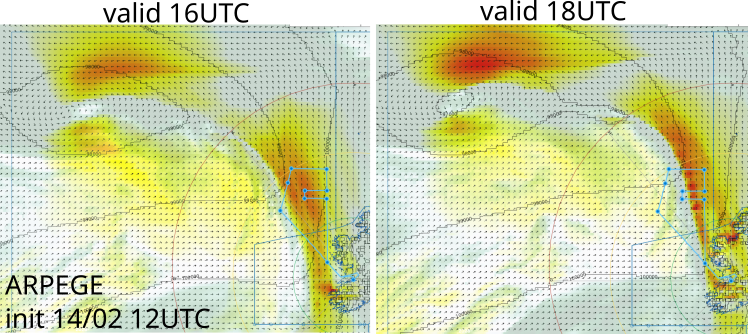
\includegraphics[width=1\linewidth]{AERIS.png}
			\caption{Wind@925hPa \& mid-level cloud cover (AERIS)}
			\label{fig:aeris1630}
		\end{figure}
		
	\end{minipage}
\vfill
\end{frame}

\begin{frame}{Boundary layer structures in SAR images?}
	\vfill
	
	\begin{minipage}{0.35\textwidth}
		\vfill
		\begin{itemize}
			\item Organized structures on sea roughness signal
			\vfill
			\item Analyses to be done to retrieve and compare to LES simulation 
		\end{itemize}
	\vfill	
	\end{minipage}
	\hfill
	\begin{minipage}{0.6\textwidth}
		\begin{figure}
		\centering
		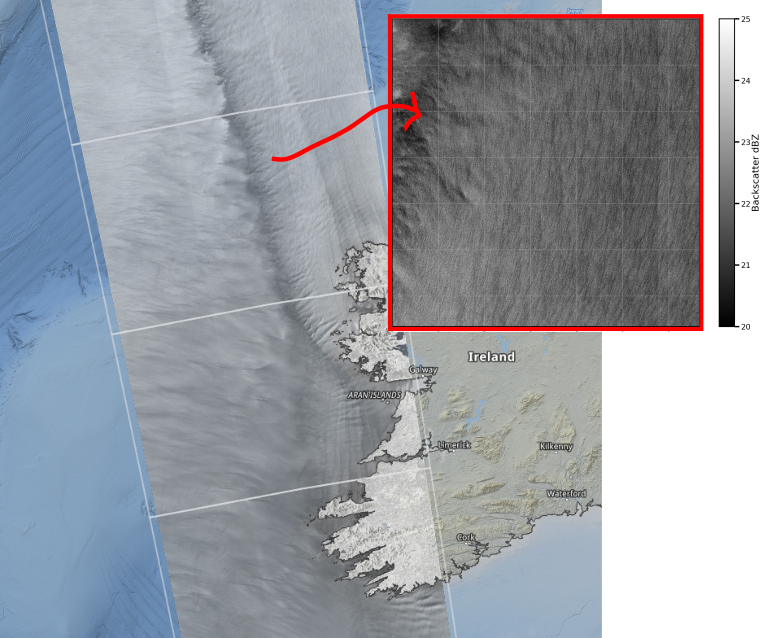
\includegraphics[width=0.9\linewidth]{sar.png}
		\caption{SAR data of S1-A at 18:03 UTC (image from ESA) }
		\label{fig:aeris1630}
		\end{figure}
		
	\end{minipage}
	\vfill
\end{frame}

\begin{frame}{Structures in the RASTA acquisition?}
Patterns in the boundary layer on the RASTA reflectivity.
		\begin{figure}
		\centering
		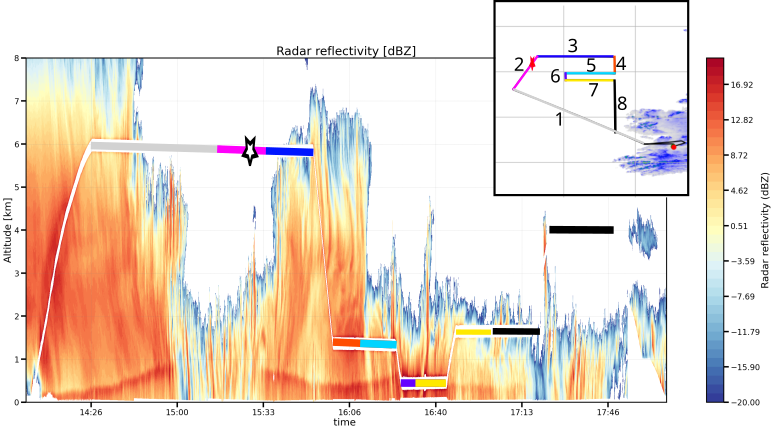
\includegraphics[width=0.75\linewidth]{RASTA_edit.png}
		\caption{RASTA reflectivity (Julien Delanoë)}
		\label{fig:aeris1630}
	\end{figure}
\end{frame}


\begin{frame}
	\vfill
Vertical wind velocity can be retrieved from the RASTA signal. 
\vfill
	\begin{figure}
		\centering
		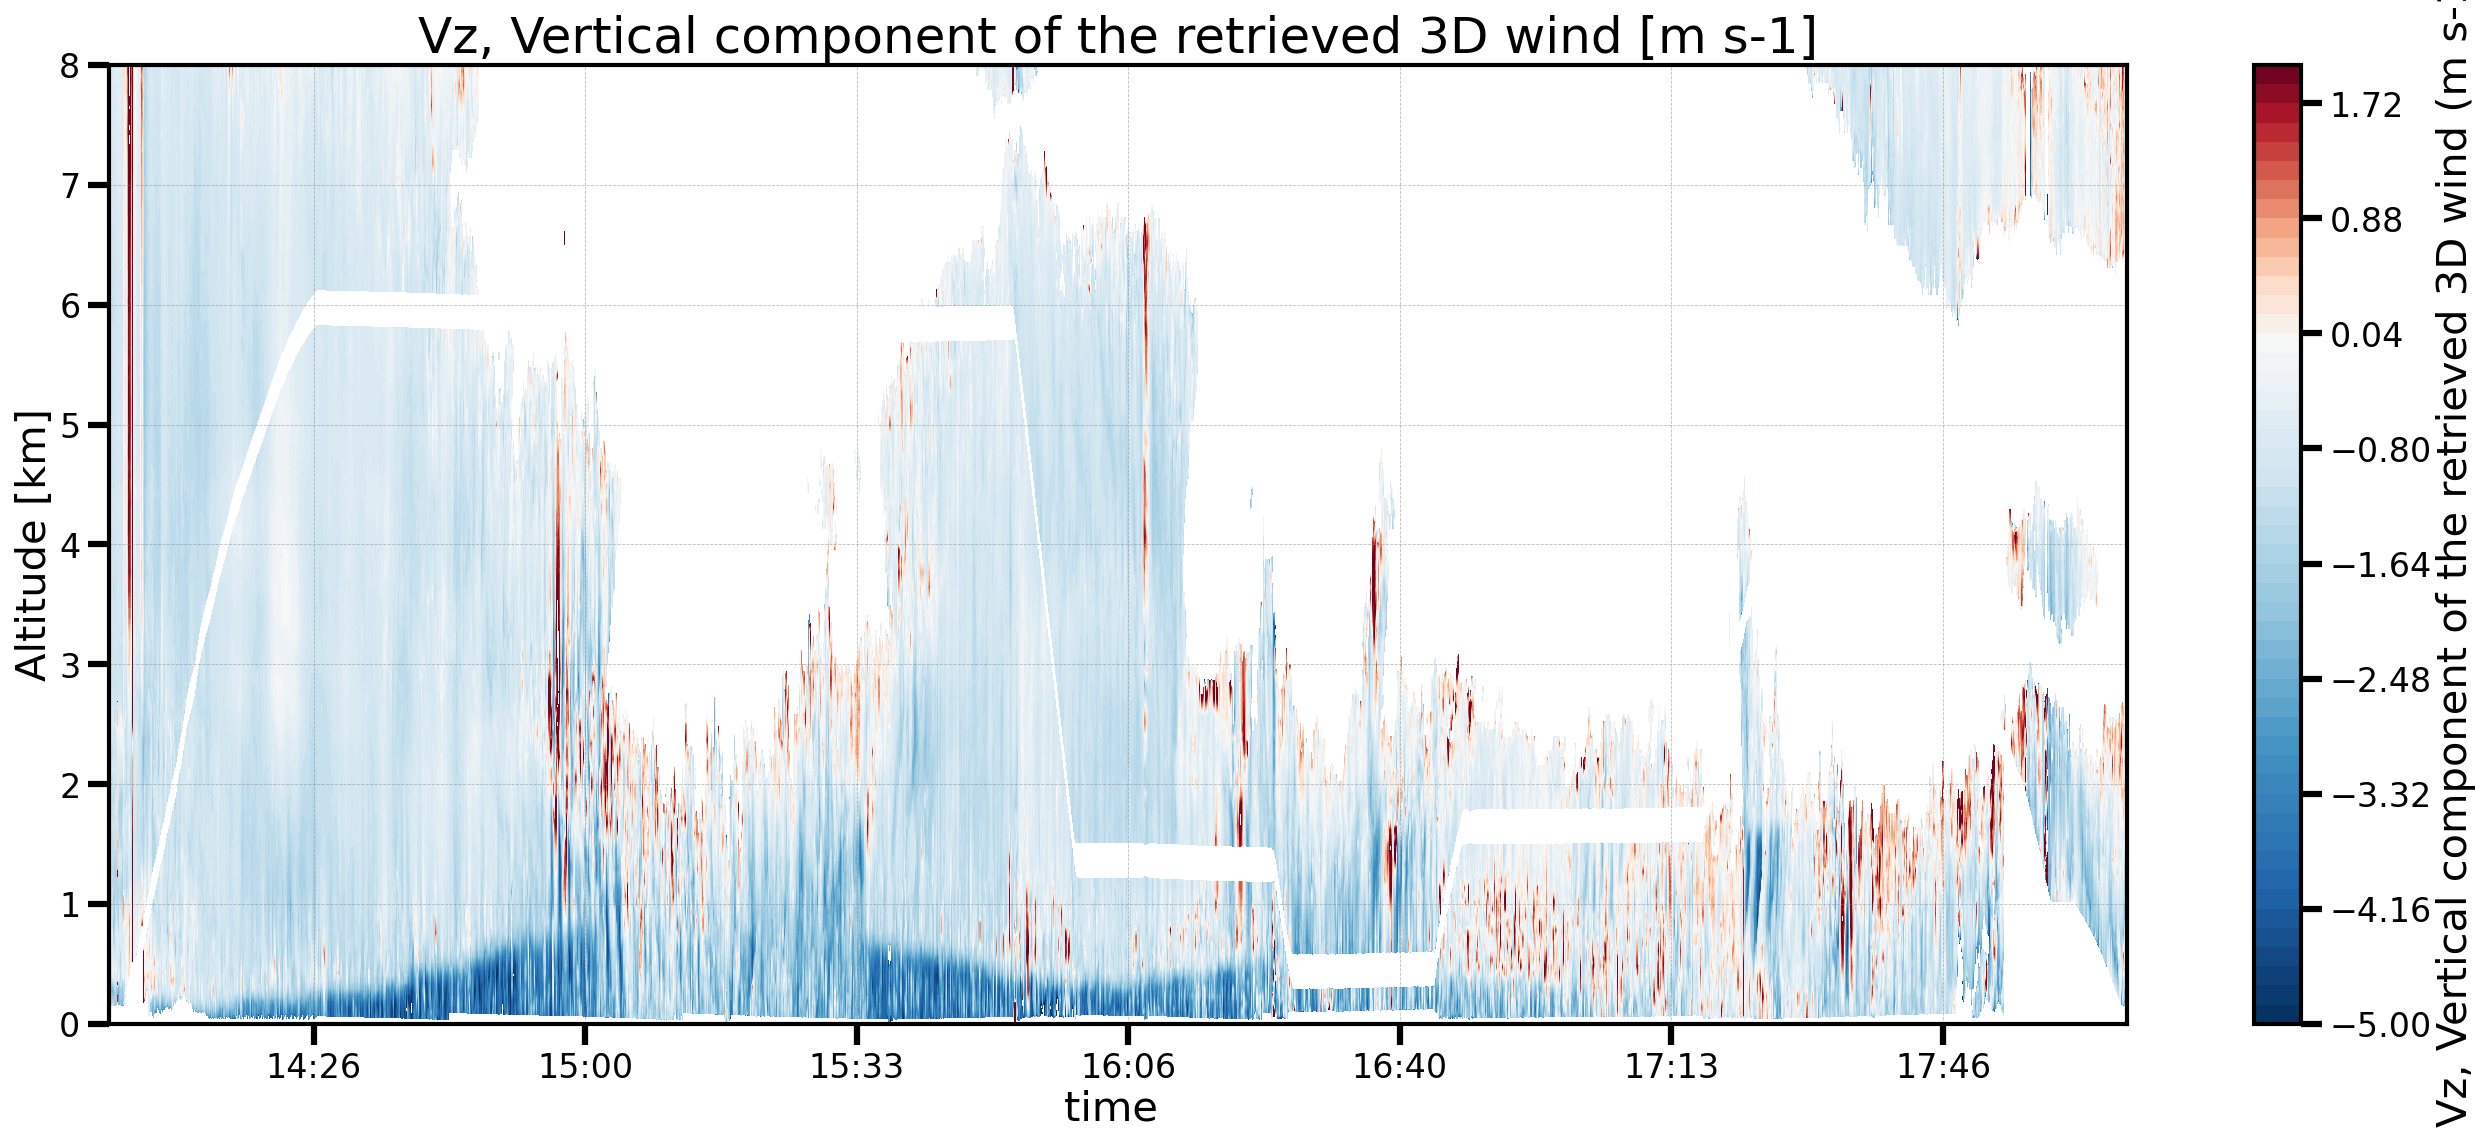
\includegraphics[width=0.8\linewidth]{RastaVZALL.png}
		\caption{RASTA W-wind (Julien Delanoë)}
		\label{fig:aeris1630}
	\end{figure}
	\vfill
\end{frame}


\begin{frame}{Special interest in the lower legs : leg 5 }
	Coherent structures detected by the RASTA (resolution 300m / 60m)? \\
	\vfill
	\begin{figure}
		\centering
		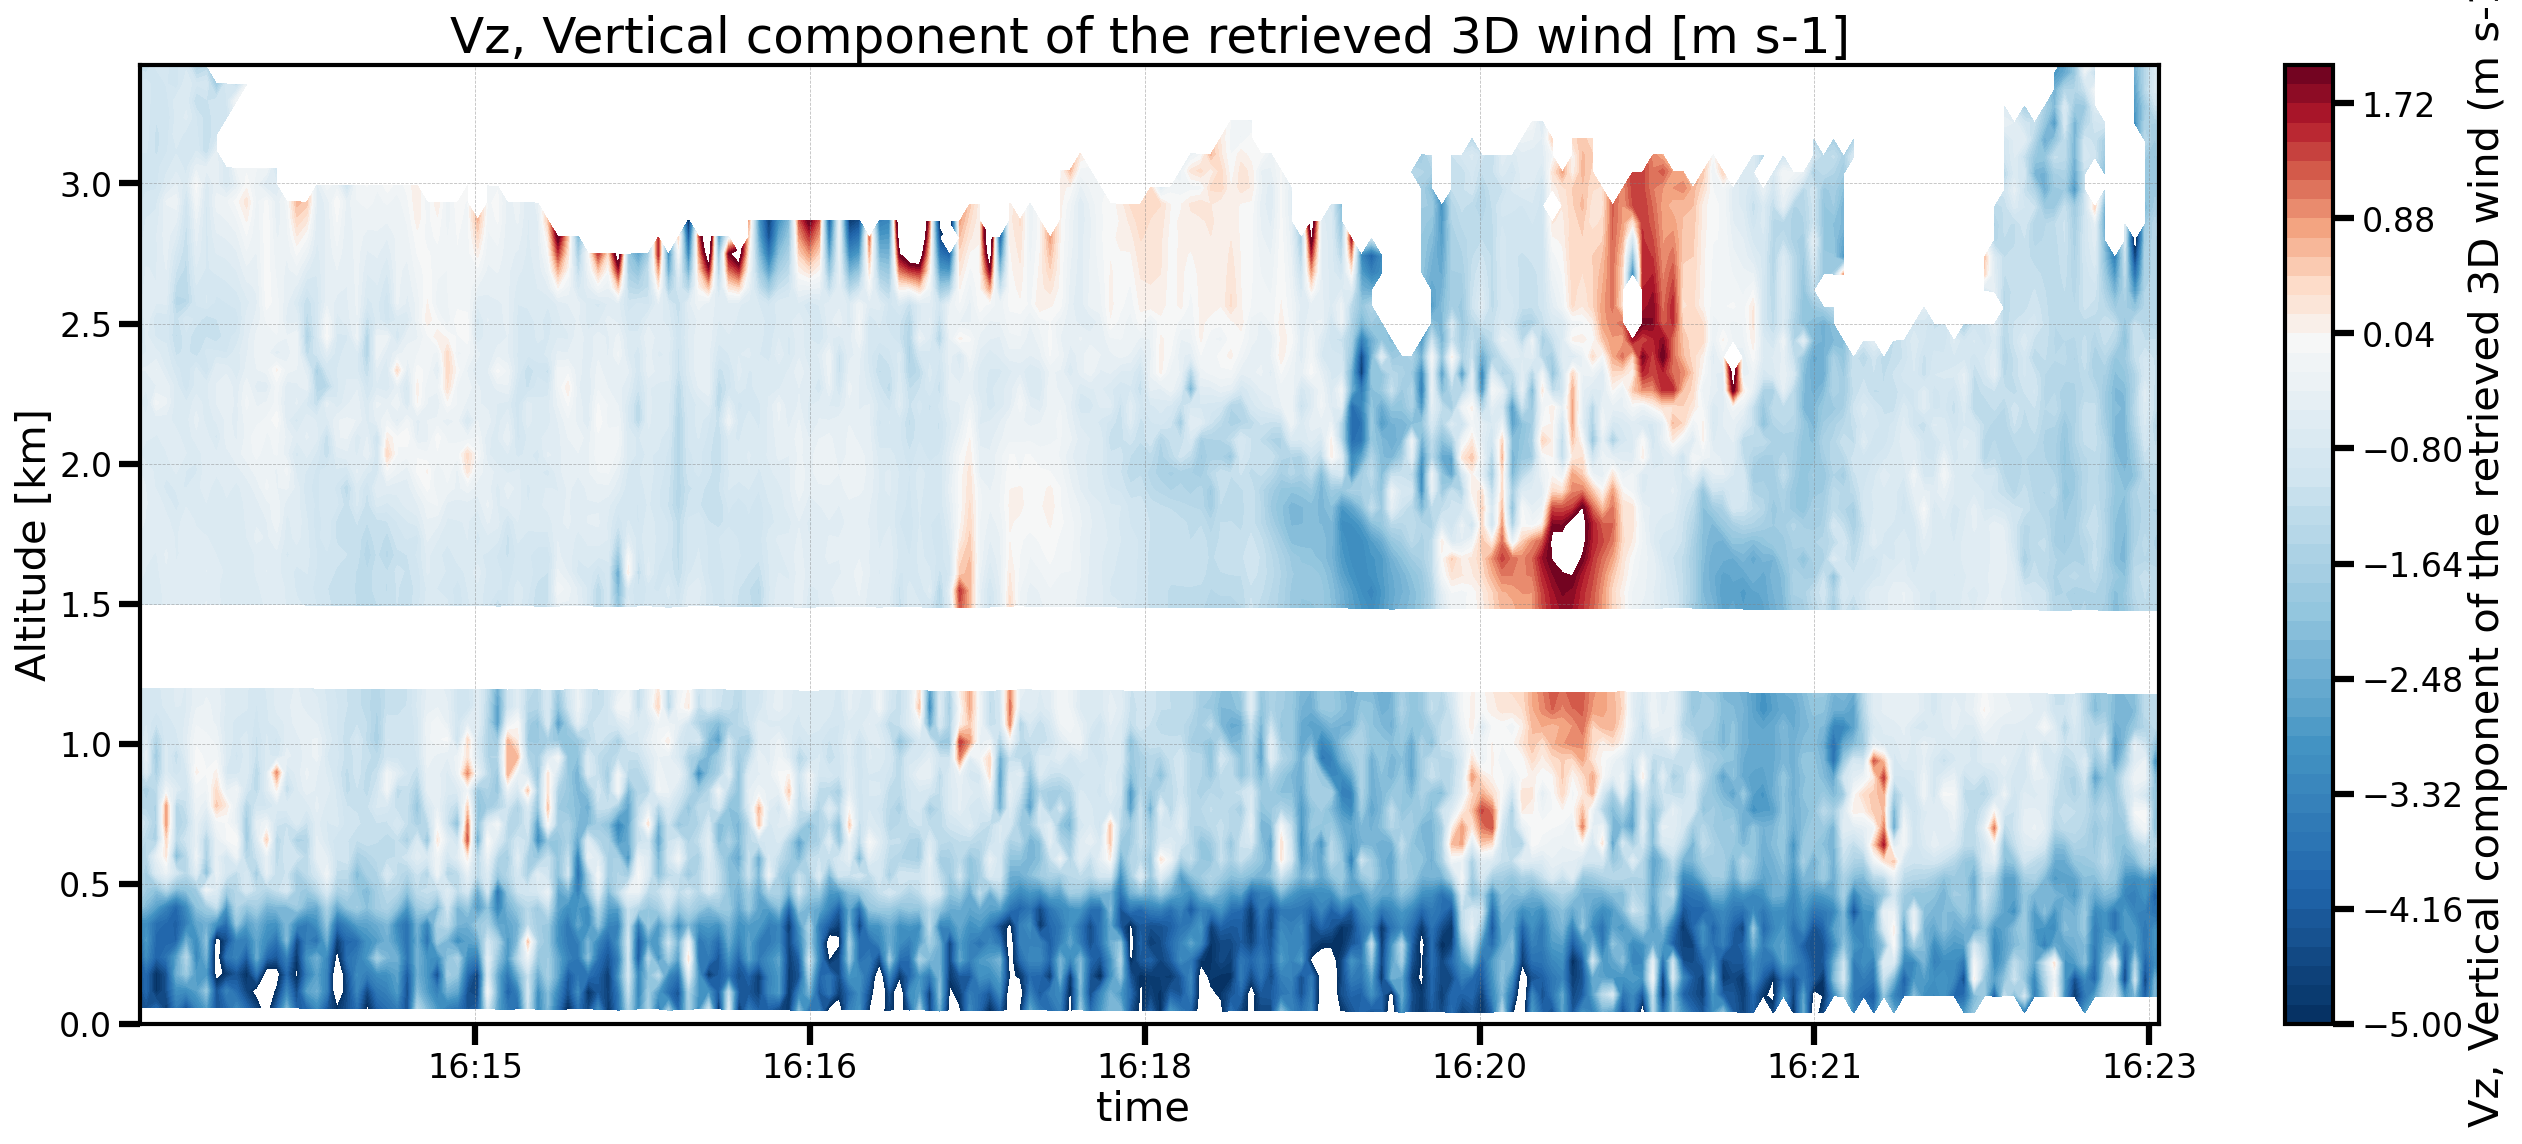
\includegraphics[width=0.8\linewidth]{RastaVZL5.png}
		\caption{W-wind retrieved from RASTA signal in legs 5  (Julien Delanoë)}
		\label{fig:aeris1630}
	\end{figure}
	\vfill
\end{frame}

\begin{frame}{Special interest in the lower legs : leg 7}
	\vfill
	Shallow convection in the leg 7. \\
	\begin{figure}
		\centering
		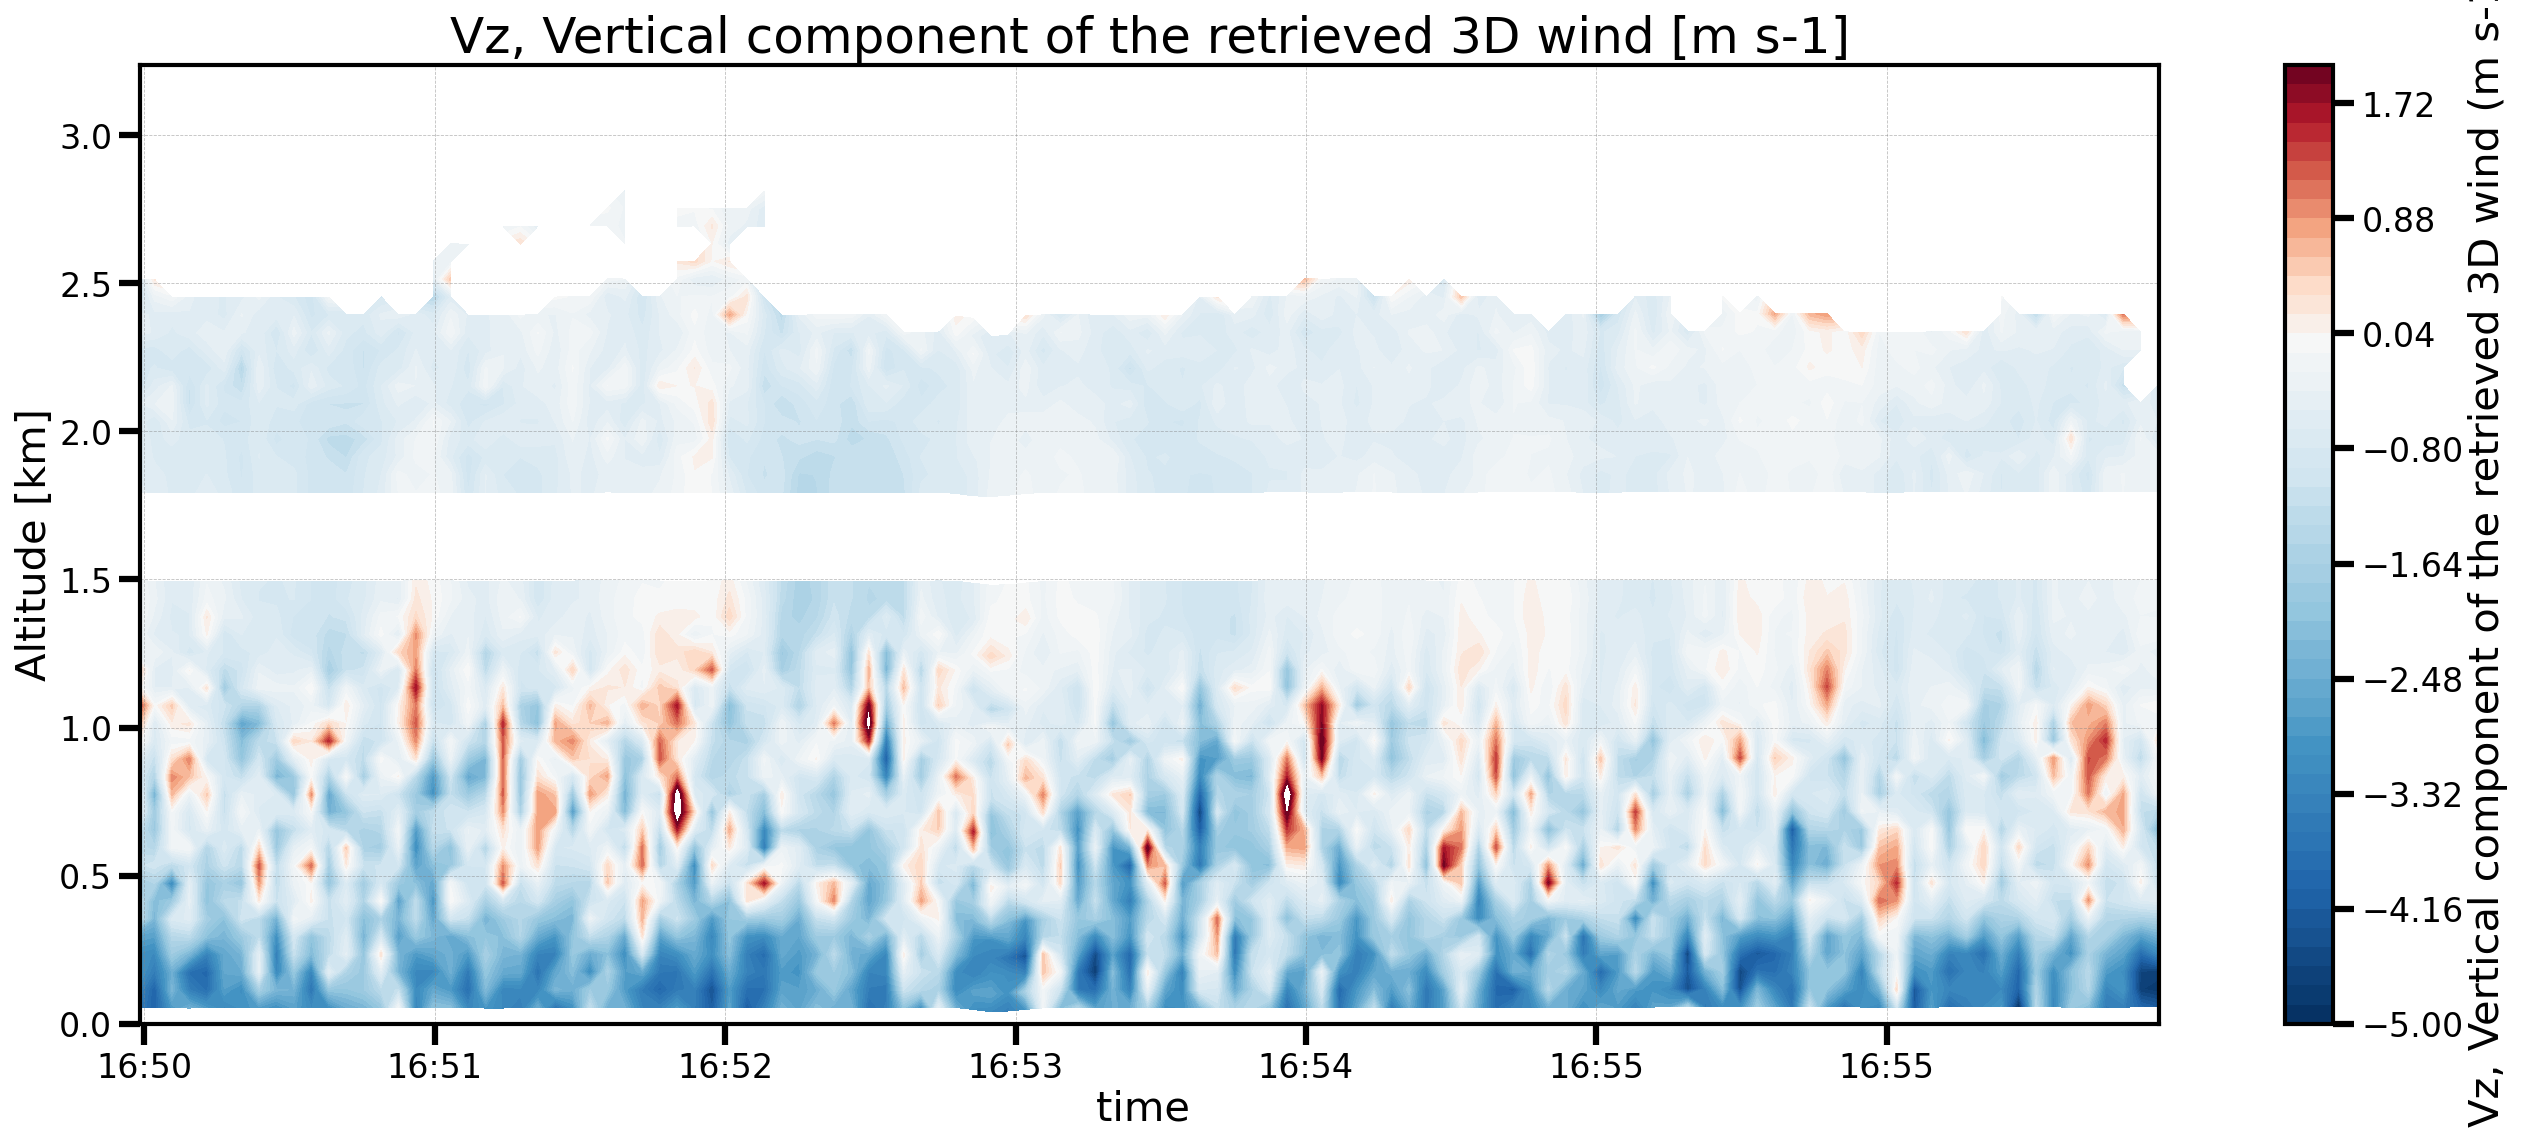
\includegraphics[width=0.8\linewidth]{RastaVZL7.png}
		\caption{W-wind retrieved from RASTA signal in legs 7  (Julien Delanoë)}
		\label{fig:aeris1630}
	\end{figure}
	\vfill
\end{frame}


\begin{frame}{Can we simulate the general situation?}
	\vfill
	
	\begin{minipage}{0.55\textwidth}
		First Meso-NH realistic simulation at a resolution of 4 km. 
		\vfill
		\begin{figure}
			\centering
			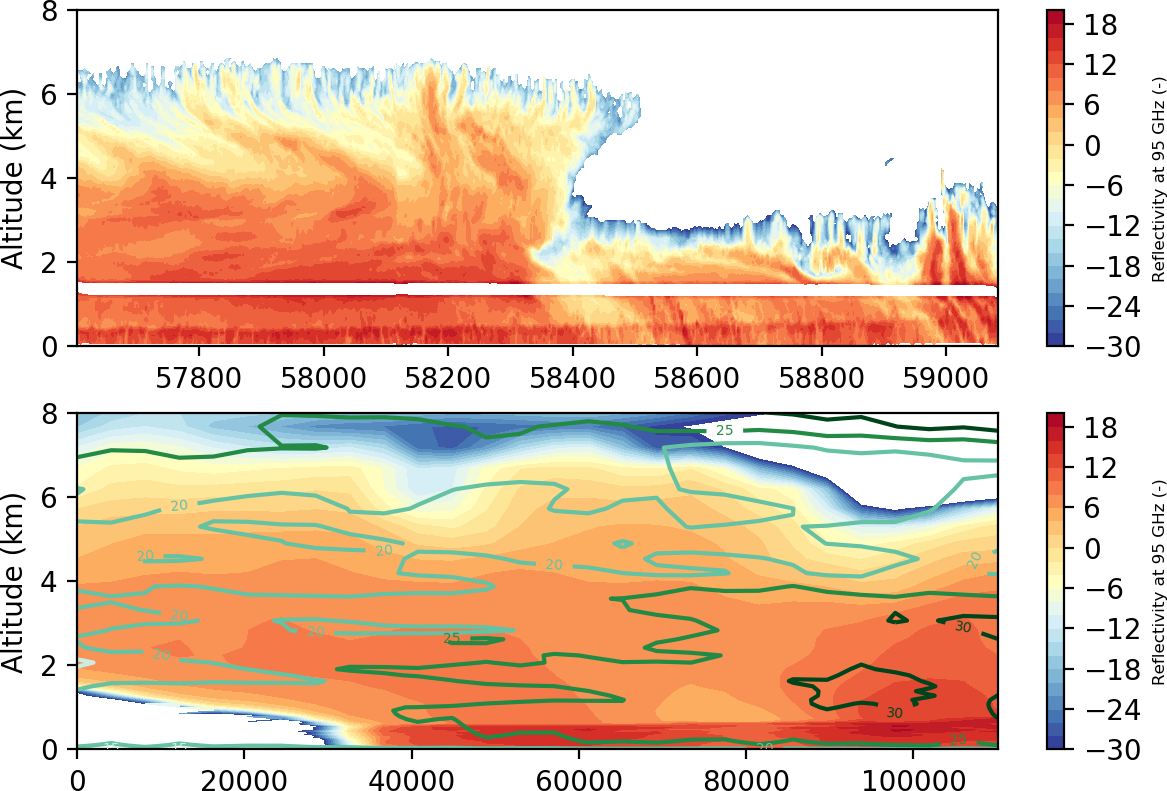
\includegraphics[width=0.7\linewidth]{FIGURES/figRASTAleg5}
			\caption{RASTA and simulation reflectivity comparison (JP Chaboureau)}
			\label{fig:figrastaleg5}
		\end{figure}
	\end{minipage}
	\hfill
	\begin{minipage}{0.4\textwidth}
		\begin{figure}
			\centering
			\animategraphics[loop, autoplay, width=0.6\textwidth]{1}{frames/frame-}{0}{8}
			\caption{$T_B$ comparison between MSG and simulation (JP Chaboureau)}
			\label{fig:aeris1630}
		\end{figure}
		
	\end{minipage}
	\vfill
\end{frame}


\begin{frame}{Hint on instabilities?}
	\vfill
	
	\begin{minipage}{0.35\textwidth}
		\vfill
		\begin{figure}
			\centering
			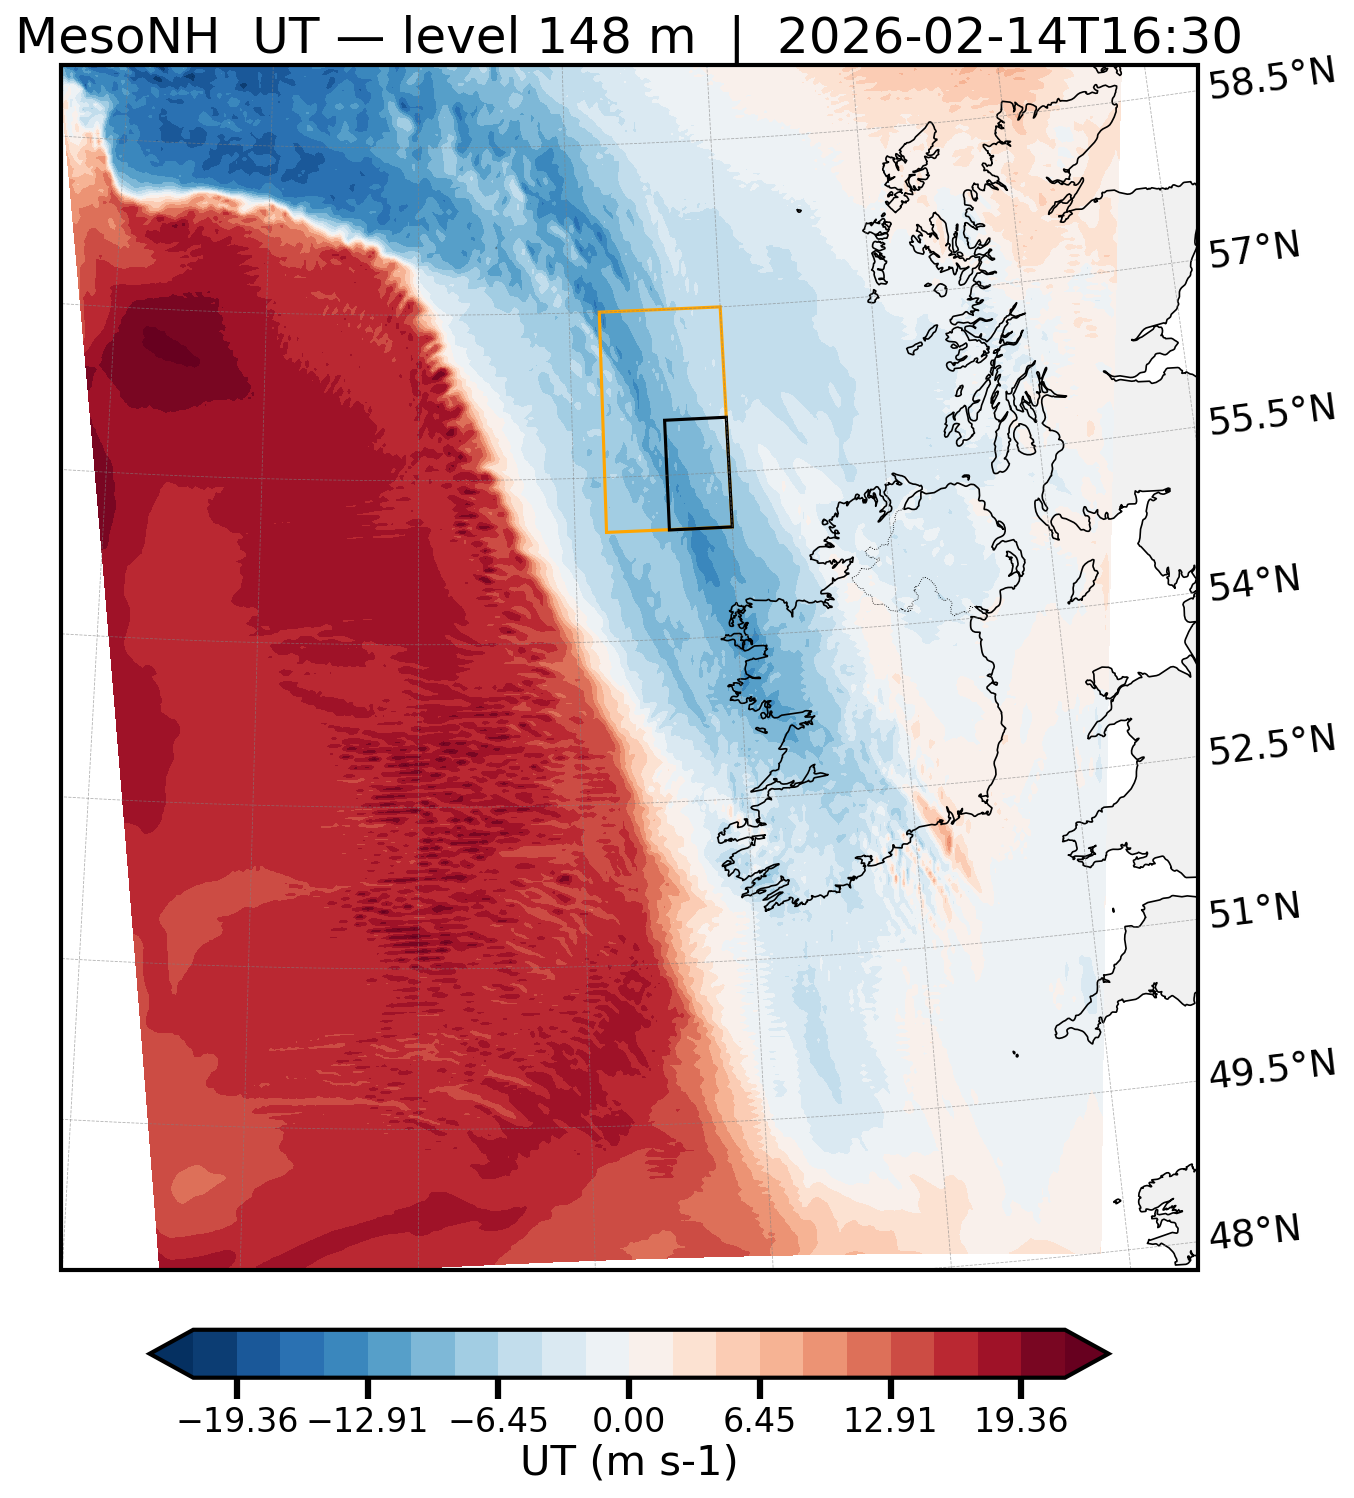
\includegraphics[width=\linewidth]{FIGURES/MNH/DOMAIN_UT_lev148.png}
			\caption{U-wind in the Meso-NH simulation}
			\label{fig:figrastaleg5}
		\end{figure}
	\end{minipage}
	\hfill
	\begin{minipage}{0.55\textwidth}
		\begin{figure}
		\centering
	
\includegraphics[width=0.8\linewidth]{FIGURES/MNH/analyse_wind.png}
	\caption{Mean wind and potential temperature profiles }
	\label{fig:figrastaleg5}
		\end{figure}
		
	\end{minipage}
	\vfill
\end{frame}

\begin{frame}{Objectives \& next steps}
The objectives of the study are :
	\vfill
\begin{itemize}
	\item to \textbf{reproduce boundary layer roll structures} and compare Meso-NH simulations with observations in RASTA and SAR
	\vfill
	\item to study the relation between the SAR signal and the 3D wind structure
	\vfill
	\item to \textbf{quantify the impact of the structures in the transport} of momentum, moisture and heat. 
\end{itemize}
\vfill
\end{frame}

\end{document}   
